\chapter{GraphQL}

\section{Entwicklung}
GraphQL ist eine Abfragesprache für APIs und Laufzeitumgebung, um auf Abfragen zu antworten~\cite{GraphQL-org}.
Seit 2012 wurde GraphQL von Facebook entwickelt und eingesetzt.
Im Jahr 2015 veröffentlichte Facebook GraphQL auf Github, wo die aktuelle Spezifikation von der GraphQL Foundation mittlerweile eigenständig weiterentwickelt wird und 2018 die letzte Version veröffentlicht wurde.
Ziel der Entwicklung war es, das Datenmodell in einer Client-Server-Anwendung durch ein Schema zu beschreiben, vom Server bereitzustellen und darauf aufbauend Abfragen zu formulieren und auszuwerten~\cite[vgl.][]{GraphQL-Spec}.
Ein Client sollte alle für eine Ansicht nötigen Daten mit einer einzigen Anfrage vom Server präzise anfordern können und daraufhin exakt diese Daten erhalten.
Das Overfetching und Underfetching von REST-APIs, d.h.\ dass ein Endpunkt mehr oder weniger Daten sendet, als benötigt werden, kann so verhindert werden, was sich besonders auf den Datenverkehr in Mobilfunknetzwerken auswirken soll.
Ein weiterer Vorteil ist die Entkopplung von den Datenbedürfnissen des Clients von den Endpunkten des Servers, wodurch getrennte Weiterentwicklung und die Wiederverwendbarkeit der API sichergestellt wird.
Die Bestandteile von GraphQL sind: \blockcquote{GraphQL-spec-github}{a type system, query language and execution semantics, static validation, and type introspection.}
Diese sollen im Folgenden erörtert werden.

\section{Spezifikation und Funktionsweise}

\subsubsection{Typsystem}
Das Schema beschreibt die API eines GraphQL-Servers durch die GraphQL Schema Definition Language (SDL).
Teil der SDL ist das Typsystem, womit ausgedrückt werden kann, welche Datenobjekte die API zur Verfügung stellt~\cite[vgl.][]{GraphQL-spec-github}.
Einstiegspunkt in das Schema bilden die drei Root-Types, welche nach Konvention \emph{query}, \emph{mutation} und \emph{subscription} genannt werden.
Alle Felder dieser drei Objekte stellen die Operationen dar, welche die API anbietet.
Unter \emph{query} werden alle Abfragetypen gesammelt, welche in einer REST-API mit GET angefragt werden würden, während zu \emph{mutation} alle Modifikationsoperationen gehören, entsprechend PUT, POST, PATCH, DELETE.
\emph{Subscription} ermöglicht es Datenströme zu senden.
Jeder Typ im Schema kann eine beliebige Zahl an Feldern enthalten, welche selbst Objekte, skalare Datentypen oder Arrays sind.
Die von GraphQL definierten skalaren Datentypen dieser Felder sind \emph{string}, \emph{int}, \emph{float}, \emph{boolean} und \emph{id}~\cite[vgl.][]{GraphQL-Spec}.
Diese können jedoch um neue Datentypen erweitert werden.
Das Typsystem erlaubt es außerdem Typen zu verbinden (Union Type) und abstrakte Typen (Interface) zu definieren, welche von konkreten Typen implementiert werden.
Jedem Feld können benannte Argumente übergeben werden, die Einfluss auf die Auswertung des Feldes haben.
\emph{Null} ist ein erlaubter Rückgabewert für alle Felder, solange diese nicht mit einem Ausrufezeichen als non-nullable gekennzeichnet werden~\cite[vgl.][]{GraphQL-Spec}.
In Abbildung~\ref{code:gql-schema} ist der Root-Query Typ mit dem Feld \emph{events} dargestellt, dem ein optionales Argument \emph{amount} mit dem Standardwert 100 übergeben wird.
Der Rückgabewert des Feldes ist ein Array, welches Eventobjekte enthält.
\begin{figure}[h]
  \centering
  \fbox{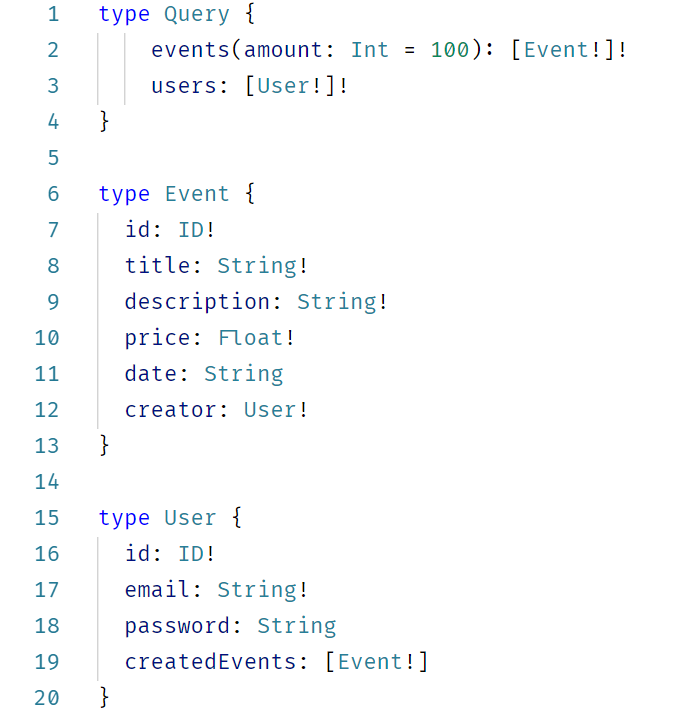
\includegraphics[width=0.6\linewidth]{graphql-schema.png}}
  \caption{GraphQL Beispielschema}\label{code:gql-schema}
\end{figure}

\begin{itemize}
  \item Query Syntax
  \begin{itemize}
    \item Abbildung Beispiel Query
    \item GraphQL Abfrage beschreibt deklarativ welche Daten erwartet werden
    \item Antwort ist üblicherweise JSON mit der gleichen Struktur
    \item Abfragen können geschachtelt werden
    \item bei Objekttyp muss mind 1 Feld angegeben werden
    \item Fragmente
    \begin{itemize}
      \item Abbildung Beispiel Fragment
      \item sammlung von Feldern von einem Typ
      \item verhindert Dopplung von mehreren Feldern in Abfrage
      \item ermöglicht typbasierte Feldselektion
    \end{itemize}
    \item mehrere gleiche queries mit alias möglich
    \item query können variablen in map übergeben werden, no manual string construction escaping
  \end{itemize}
  \item Introspektion
  \begin{itemize}
    \item Spezialfelder beginnend mit doppelt Unterstrich
    \item \_\_schema, \_\_typename
    \item Metadaten über GraphQL Schemas
    \item Sinn ist Nutzung durch Entwicklungstools
    \item ermöglicht statische Validierung: GraphQL Abfrage kann zu Entwicklungszeit geprüft werden
  \end{itemize}
  \item Referenzen werden unsichtbar, da von GraphQL Server automatisch aufgelöst (Performance beachten!)
  \item ein Endpunkt (kein Nutzen von URIs)
  \item jede Abfrage mit POST (kein Nutzen von HTTP Methoden), query in query feld in json payload
  \item immer 200 OK status code
  \item keine URI nutzung -> level 0 mmr
  \item application/graphql media type
  \item nicht im Spec festgelegt (da netzwerkunabhängig), aber praxis
  \item Semantik der Abfrage von Server ausgewertet (welche der CRUD Operationen)
\end{itemize}

% \begin{figure}[h]
%   \centering
%   \fbox{\includegraphics[width=\linewidth]{}}
%   \caption{REST~\cite[84]{REST}}\label{img:REST-diss}
% \end{figure}

\begin{figure}[h]
  \centering
  \begin{minted}{http}
    HTTP/1.1 200 OK
  
    {
      book: {
        id: 1,
        title: "REST in practice",
        author: "http://api.com/author/10",
        coverImage: "http://api.com/books/1/cover.jpg",
        reviews: "http://api.com/books/1/reviews?first=10",
        relatedBooks: [
          "http://api.com/books/14"
        ],
        next: "http://api.com/books/2",
      }
    }
  \end{minted}
  \caption{Level 3 Hypermedia JSON Response}\label{code:lvl3}
\end{figure}

\section{Server-Execution}
\begin{itemize}
  \item request empfangen
  \item lexing: zeichenstream in graphql tokens umgewandelt
  \item parsing: semantik korrekt, struktur
  \item lexer und parser algorithmus nicht im spec festgelegt
  \item ermöglicht spezifische optimierungen
  \item server validiert query mit schema, inputvalidierung
  \item validierungsregeln im spec oder selbst festgelegt:
  \item validierung erfolgt depth first
  \item query Feld für Feld parallel ausgeführt
  \item jedes Feld hat eigenen resolver
  \item resolver für jedes Feld aufgerufen
  \item resolver erfüllen wert nach schema
  \item breadth-first (Abbildung), 3 und 4 parallel
  \item parent result an child resolver weitergegeben
  \item Felder in manchen Implementierungen als trivial automatisch aufgelöst
  \item rückgabewert der Felder an Schema geprüft, evtl konvertiert
  \item JSON kennt nur number, nicht int und float
  \item graphql sendet nie etwas was nicht im schema ist
\end{itemize}